\documentclass[a4paper, 12pt, titlepage]{report}

%Taal: Nederlands ("Inhoudsopgave", "Hoofdstuk",...)
\usepackage{graphicx}
\usepackage{subcaption}
\usepackage{algorithmic}
\usepackage{amsmath, amssymb, textcomp, mathtools}

%Geen nummering bij secties en hoofdstukkden
\setcounter{secnumdepth}{-1} 

%geen indents
\setlength\parindent{0pt}

\usepackage[dutch]{babel}
\begin{document}

\title{\textbf{Numerieke Modellering en Benadering}\\\textit{Practicum 1: Eigenwaardenproblemen}\\}
\author{De Wolf Peter\\ Vekemans Wout}

\date{\today}
\begin{titlepage}
	\maketitle
	\thispagestyle{empty}
\end{titlepage}

\newpage

\listoffigures

\newpage

\section{Inleiding}
In dit practicum onderzoeken we methoden voor het bepalen van eigenwaarden van vole matrices. In een eerste sectie beschouwen we enkele theoretische eigenschappen van de methoden. In een tweede sectie worden de convergentie-eigenschappen van da methoden onderzocht aan de hand van MATLAB-experimenten. In de derde en laatste sectie gaan we dieper in op \'e\'en van de methoden, namelijk de Jacobi-methode.
\section{Theoretische eigenschappen}

\subsection{Opgave 1}

\subsection{Opgave 2}

\section{Convergentie-experimenten}
Voor al deze experimenten wordt gebruik gemaakt van een volle, re\"ele symmetrische matrix A. We laden hiervoor de gegeven matrix $mat1.txt$ in in MATLAB.

\subsection{Opgave 4}
Het uitvoeren van het $spy$-commando laat zien dat er geen enkel $non-zero$ element in de matrix zit. De uitvoering van het QR-algoritme op een matrix met die afmetingen (nog steeds relatief klein) zou zeer veel werk vragen. \\
Na het reduceren tot Hessenberg vorm zien we dat alle elementen onder de eerste benedendiagonaal nul zijn geworden. Verdere analyse leert ons dat ook de elementen boven de eerste bovendiagonaal allemaal van grootteorde $\epsilon_{mach}$ zijn. Als we de Hessenberg vorm van de matrix afronden tot op 15 decimalen verkijgen we een tridiagonale matrix.(zie figuur \ref{hessenberg}) Dit komt doordat de originele matrix symmetrisch was. De reductie naar Hessenberg vorm zorgt ervoor dat het algoritme niet op een volledige matrix moet inwerken. Het uitvoeren van het QR-algoritme vraagt nu slechts $\mathcal{O}(n^2)$ flops. 
\begin{figure}[!h]
\begin{subfigure}{.5\textwidth}
\centering
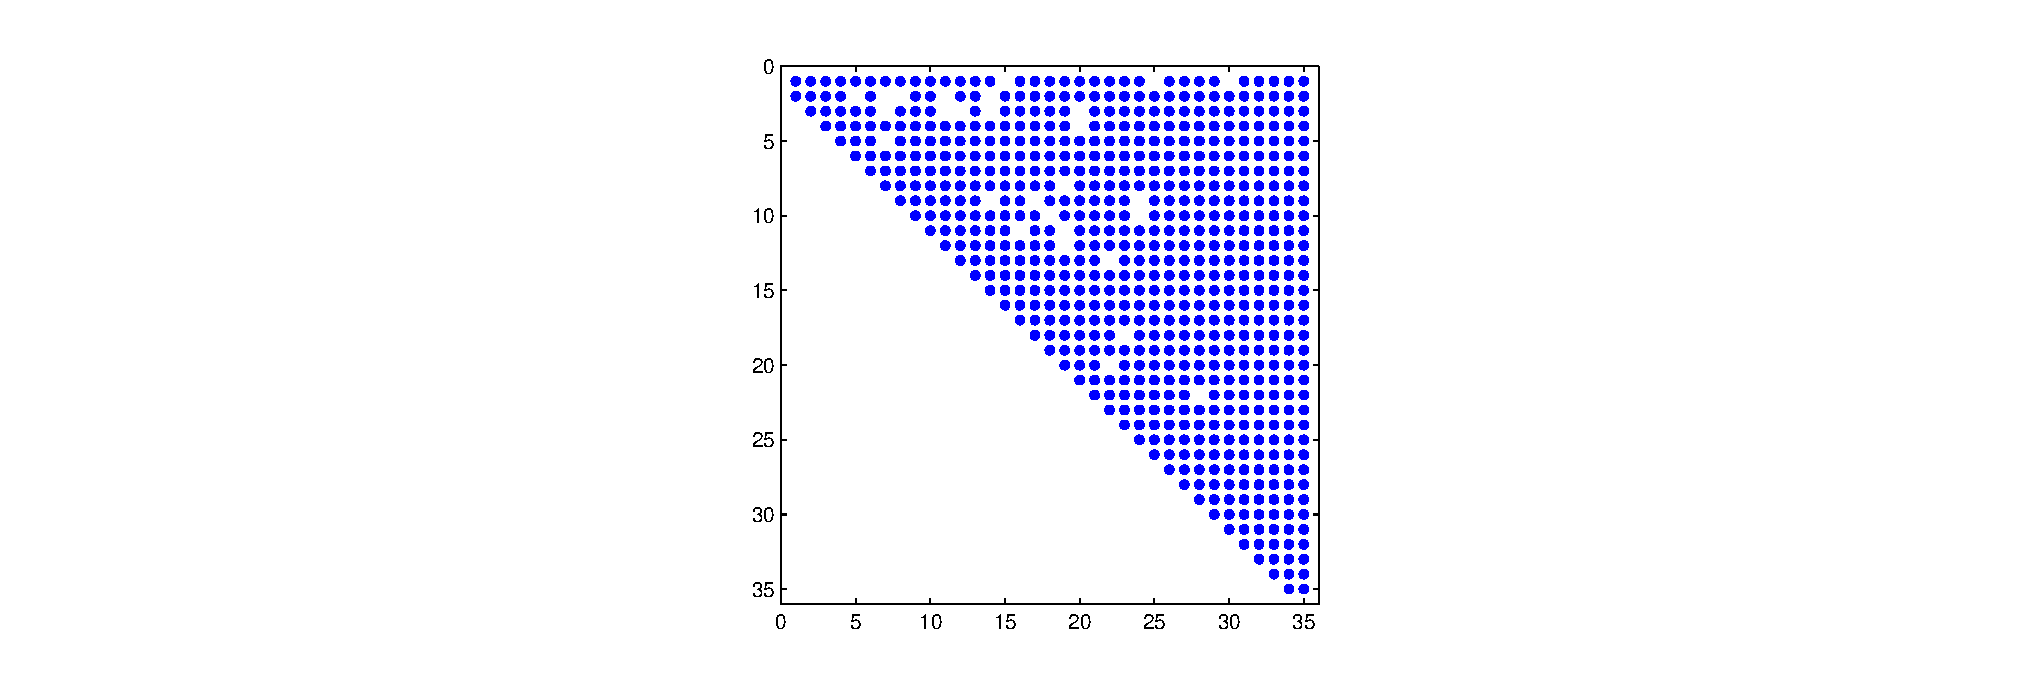
\includegraphics[width=\textwidth]{structuur_hessenberg.eps}
\subcaption{zonder afronden}
\end{subfigure}
\begin{subfigure}{.5\textwidth}
\centering
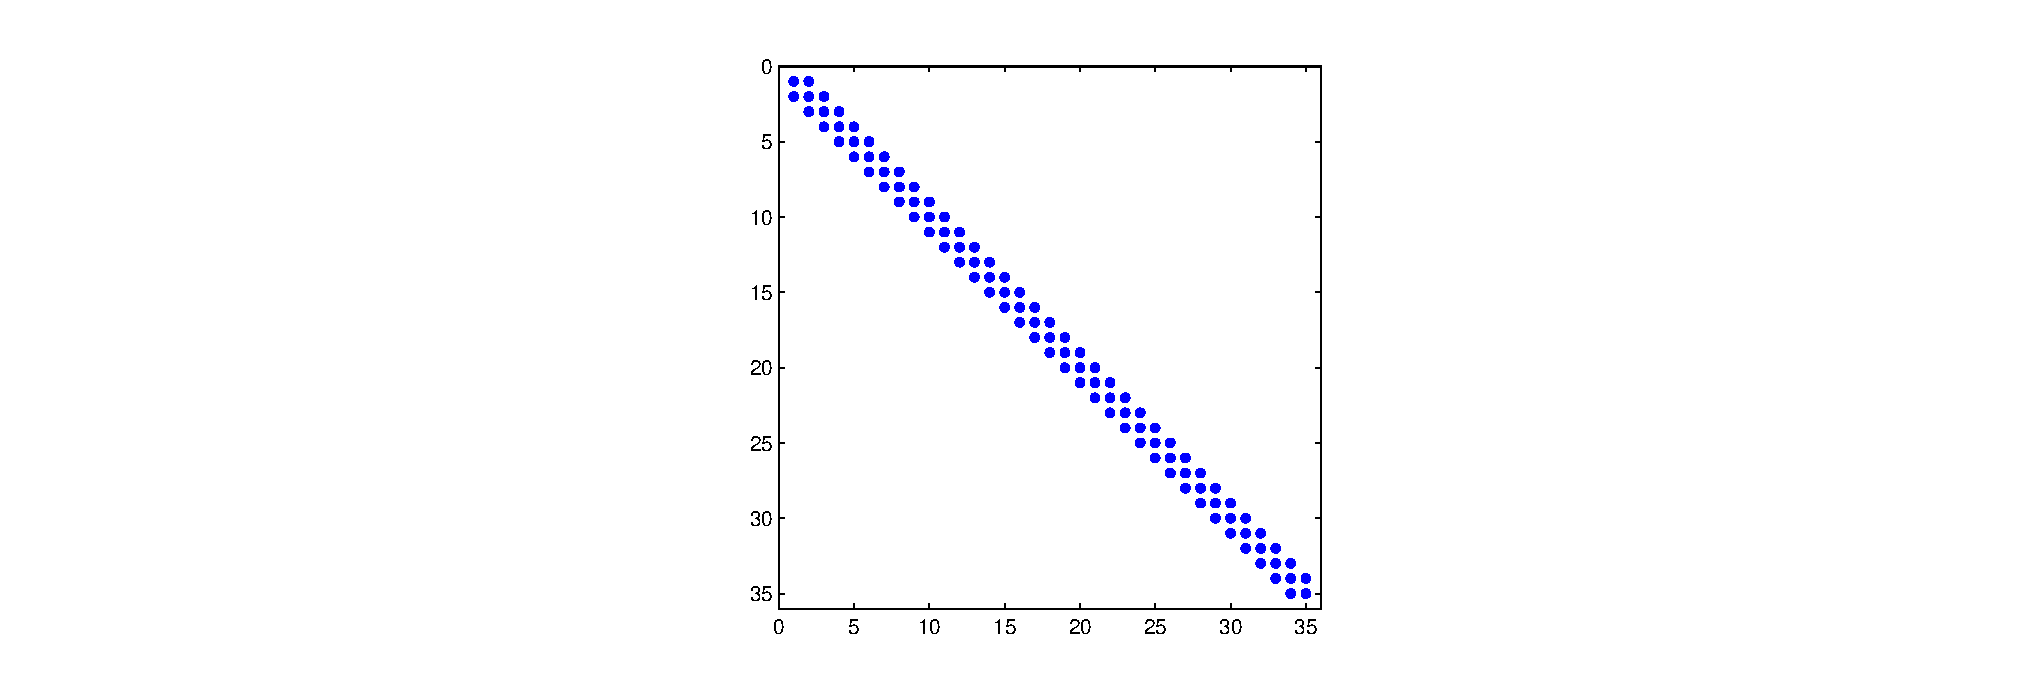
\includegraphics[width=\textwidth]{afgerond.eps}
\subcaption{met afronden}
\end{subfigure}

\caption{Structuur van de Hessenberg matrix}
\label{hessenberg}
\end{figure}

\subsection{Opgave 5}
Na uitvoeren van de drie methoden verkrijgen we ...... TODO we zien duidelijk dat het QR-algoritme zonder shifts een lineaire convergentie heeft. \\

Als maat voor de convergentie gebruiken we de relatieve fout op de berekende eigenwaarden. 

Voor het algoritme zonder shifts stemt dit volledig overeen met de theorie. Theorem 28.4 (p. 218 in het handboek) geeft duidelijk aan dat bij het gebruik van QR zonder shifts $A^{(k)}$ lineair convergeert naar een diagonaalmatrix met de eigenwaarden van $A$ als elementen.In Tabel \ref{errorNoShift} staan de relatieve fouten op de vijf dominante eigenwaarden van de matrix, bij gebruik van het algoritme zonder shifts. Zie ook figuur \ref{graphNoShift} voor een grafische illustratie van de convergentie.\\
\begin{center}
\begin{table}

\begin{tabular}{r||r|r|r|r|r}

Iteratie & 23 & 22& 21&20&19 \\
\hline
5	&	3.4173E-02	&	7.7106E-02	&	7.8187E-02	&	6.4348E-02	&	1.6090E-02	\\
10	&	1.7414E-02	&	1.5644E-02	&	5.4016E-02	&	2.7533E-02	&	3.4097E-03	\\
15	&	1.1828E-02	&	7.6086E-03	&	2.5512E-02	&	2.6705E-02	&	1.8666E-02	\\
20	&	8.1546E-03	&	7.6596E-03	&	1.4755E-02	&	1.9487E-02	&	2.2061E-02	\\
25	&	5.5253E-03	&	5.5328E-03	&	9.3537E-03	&	1.1783E-02	&	1.6347E-02	\\
30	&	3.6818E-03	&	3.7494E-03	&	5.9809E-03	&	7.2101E-03	&	1.1119E-02	\\
35	&	2.4229E-03	&	2.4821E-03	&	3.7863E-03	&	4.3930E-03	&	7.2111E-03	\\
40	&	1.5805E-03	&	1.6235E-03	&	2.3726E-03	&	2.6464E-03	&	4.5407E-03	\\
45	&	1.0249E-03	&	1.0543E-03	&	1.4757E-03	&	1.5767E-03	&	2.8068E-03	\\
50	&	6.6195E-04	&	6.8157E-04	&	9.1340E-04	&	9.3132E-04	&	1.7155E-03	\\
55	&	4.2643E-04	&	4.3936E-04	&	5.6357E-04	&	5.4674E-04	&	1.0413E-03	\\
60	&	2.7425E-04	&	2.8270E-04	&	3.4703E-04	&	3.1955E-04	&	6.2951E-04	\\
65	&	1.7618E-04	&	1.8169E-04	&	2.1342E-04	&	1.8615E-04	&	3.7964E-04	\\
70	&	1.1310E-04	&	1.1668E-04	&	1.3115E-04	&	1.0814E-04	&	2.2861E-04	\\
75	&	7.2573E-05	&	7.4891E-05	&	8.0558E-05	&	6.2672E-05	&	1.3754E-04	\\
80	&	4.6554E-05	&	4.8055E-05	&	4.9466E-05	&	3.6236E-05	&	8.2704E-05	\\
85	&	2.9857E-05	&	3.0829E-05	&	3.0368E-05	&	2.0900E-05	&	4.9712E-05	\\
90	&	1.9147E-05	&	1.9775E-05	&	1.8641E-05	&	1.2024E-05	&	2.9873E-05	\\
95	&	1.2277E-05	&	1.2683E-05	&	1.1442E-05	&	6.8983E-06	&	1.7948E-05	\\

\end{tabular}
\caption{Relatieve fout op de vijf grootste berekende eigenwaarden (zonder shifts)}
\label{errorNoShift}
\end{table}
\end{center}



\subsection{Opgave 6}
De Rayleigh quoti\"ent iteratie en de Rayleigh shift methode zouden allebei kubisch moeten convergeren. In figuur \ref{vglRayleigh} zijn onze numerieke bevindingen weergegeven. We zien duidelijk dat er een gelijkaardige convergentiesnelheid is. Dit komt doordat de Rayleigh shift methode gebruik maakt van het Rayleigh quoti\"ent. Het QR algoritme met Rayleigh shifts is namelijk een methode waarbij er snelle convergentie is in de laatste kolom van $Q^{(k)}$. Het Rayleigh quoti\"ent $\mu^{(k)}$ van de laatste kolom van de matrix is dan een goede schatting voor de eigenwaarde horende bij de laatste kolom. 
\begin{equation}
	\mu^{(k)} = \frac{(q^{(k)}_m)^TAq^{(k)}_m}{(q^{(k)}_m)^Tq^{(k)}_m} = (q^{(k)}_m)^TAq^{(k)}_m
	\label{eqn:rayleighquotient}
\end{equation}
Nu is dit getal gelijk aan $A^{(k)}_{mm}$ en kan dit getal zo als shift gebruikt worden voor de volgende iteratiestap.\\

De convergentie van gelijktijdige iteratie en QR zonder shifts wordt ge\"illustreerd in figuur \ref{vglSimQR}. Als residu gebruiken we hier de relatieve fout op de diagonaal van A. Dit kan een licht vertekend beeld geven als er enkele eigenwaarden niet zo snel convergeren, maar voor een globaal beeld is het voldoende. Het is duidelijk dat deze methodes ongeveer even snel convergeren. Dit kan eenvoudig worden aangetoond. Het algoritme voor gelijktijdige iteratie is als volgt:

\begin{algorithmic}
 \STATE Kies $\hat{Q}^{(0)}\in \mathbb{R}^{m\times n}$ met orthonormale kolommen
 \FOR{$k=1,2,...$} 
 	\STATE $Z = A\hat{Q}^{(k-1)}$
 	\STATE $\hat{Q}^{(k)}\hat{R}^{(k)} = Z$
 \ENDFOR
\end{algorithmic}

Theorema 28.3 (p. 216) in het handboek toont aan dat gelijktijdige iteratie en unshifted QR dezelfde matrices $\underline{R}^{(k)},\underline{Q}^{(k)} en \underline{A}^{(k)}$ genereren. Het is ook eenvoudig in te zien dat dit de matrices zijn die gedefinieerd worden door de $k^{de}$ macht van de QR factorisatie van $A$.\\

Volgens theorema 28.4 (p. 218) convergeert het QR algoritme zonder shifts lineair naar een diagonaalmatrix. Aangezien gelijktijdige iteratie dezelfde matrices produceert moet deze methode een gelijkaardige convergentiesnelheid hebben. Uit figuur \ref{vglSimQR} wordt duidelijk dat matrix A inderdaar lineair convergeert naar een diagonaalmatrix.


\begin{figure}[htb]
	\centering
	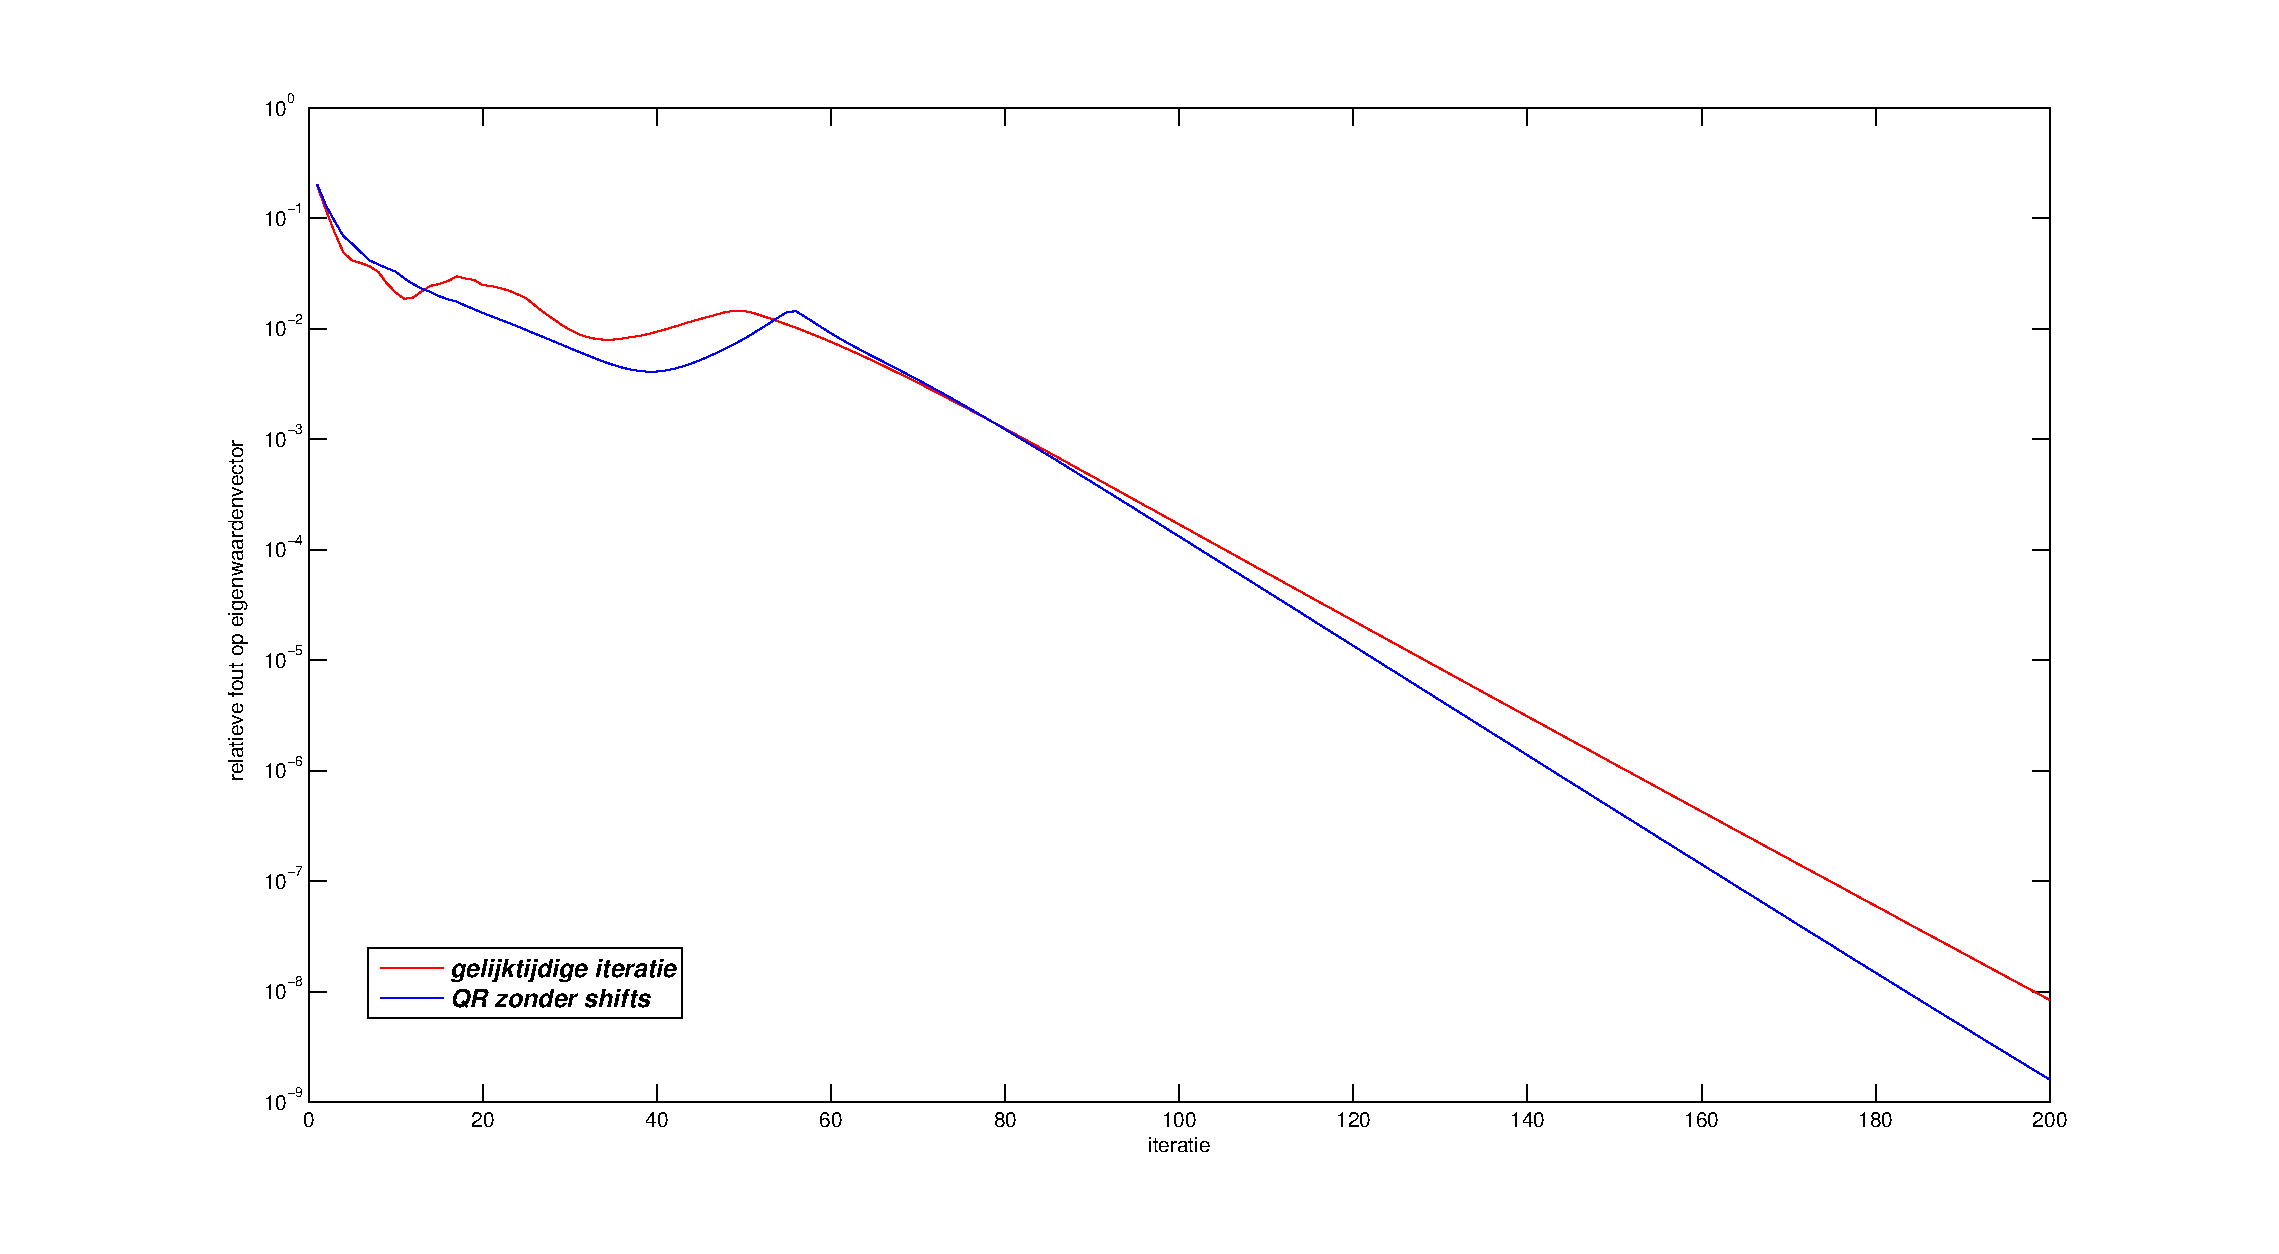
\includegraphics[width=0.8\textwidth]{vergelijkingLineair.eps}
	\caption{Vergelijking convergentie van unshifted QR en gelijktijdig iteratie}
	\label{vglSimQR}
\end{figure}


\subsection{Opgave 7}

\section{Alternatieve eigenwaardenalgoritmen}

\subsection{Opgave 8}

\subsection{Opgave 9}

\subsection{Opgave 10}

\end{document}
